\chapter{Аналитическая часть}
\section{Оптические эффекты, учитываемые при построении реалистичного изображения}
При построении реалистичных изображений необходимо учитывать такие эффекты оптики, как:
\begin{itemize}
	\item отражающие свойства поверхностей: диффузное и зеркальное отражения;
	\item преломление части света при взаимодействии луча с прозрачной поверхностью;
	\item рассеяние света.
\end{itemize}

Поскольку в данной работе не используются прозрачные объекты, будем рассматривать только отражение и рассеяние света.

Диффузная составляющая явления отражения света от поверхностей описывается следующим уравнением:
\begin{equation}
	I_\text{д} = I_\text{и} cos\theta \cdot k_\text{д}, 
\end{equation}
где $I_\text{и}$ -- интенсивность источника освещения, $\theta$ – угол между нормалью к поверхности в точке отражения и вектором, направленным из точки отражения к источнику света, $k_\text{д}$ -– коэффициент диффузного отражения.

Зеркальная составляющая явления отражения света описывается уравнением:
\begin{equation}
	I_\text{з} = I_\text{и} cos^n\alpha \cdot k_\text{з}, 
\end{equation}
где $I_\text{и}$ -- интенсивность источника освещения, $\alpha$ -- угол падения луча, $k_\text{з}$ -- коэффициент зеркального отражения, степень $n$ косинуса характеризует концентрированность света в направлении отражения.

Рассеяние света в компьютерной графике обычно описывают следующей формулой:
\begin{equation}
	I' = I_\text{р}k_\text{р}, 
\end{equation}
где $I_\text{р}$ -- интенсивность рассеянного света, $k_\text{р}$ -- коэффициент диффузного отражения рассеянного света.

Также необходимо учесть затухание света с расстоянием. Интенсивность света падает обратно пропорционально квадрату расстояния до источника, однако, как показывает практика, большей реалистичности можно добиться при линейном затухании \cite{lit1}. В этом случае получаем следующий результат:
\begin{equation}
	I = I_\text{р}k_\text{р} + \frac{I_\text{и} cos\theta \cdot k_\text{д} + I_\text{и} cos^n\alpha \cdot k_\text{з}}{d + K}, 
\end{equation}
где $d$ -- расстояние до источника освещения, $K$ -- произвольная константа.

\section{Алгоритмы удаления невидимых линий и поверхностей}
Все алгоритмы удаления невидимых линий работают либо в пространстве объектов, либо в пространстве изображений. Рассмотрим наиболее известные из них~\cite{lit1}.
\subsection{Алгоритм Робертса}
Этот алгоритм работает в объектном пространстве и использует проекции объектов на картинную плоскость для анализа видимости. Алгоритм прежде всего удаляет из каждого тела те ребра или грани, которые экранируются самим телом. Затем каждое из видимых ребер каждого тела сравнивается с каждым из оставшихся тел для определения того, какая его часть или части, если таковые есть, экранируются этими телами. Поэтому вычислительная трудоемкость алгоритма Робертса растет теоретически как квадрат числа объектов~\cite{lit1}.

\subsection{Алгоритм Варнока}
Алгоритм Варнока основывается на рекурсивном разбиении окна на подокна всякий раз, когда оно не пусто, до окна размеров в 1 пиксель, после чего определяется ближайший к наблюдателю объект, пиксель закрашивается цветом этого объекта. Рекурсивность алгоритма является главным недостатком алгоритма: окно каждый раз делится на 4 подокна, если размер окна больше одного пикселя, или оно содержит несколько объектов, или пересекается с объектом.

\subsection{Алгоритм, использующий z-буфер}

Алгоритм основывается на хранении глубины (z-значения) каждого пикселя экрана и определении ближайшей к экрану точки при разложении многоугольников в растр.
Главное преимущество алгоритма -- его простота. Кроме того, этот алгоритм решает задачу об удалении невидимых поверхностей и делает тривиальной визуализацию пересечений сложных поверхностей -- сцены могут быть любой сложности.
Основной недостаток алгоритма -- большой объем требуемой памяти \cite{lit1}.


\subsection{Алгоритм обратной трассировки лучей}
Метод прямой и обратной трассировки лучей заключается в том, что от момента испускания лучей источником света до момента попадания в камеру, траектории лучей отслеживаются, и рассчитываются пересечения лучей с лежащими на траектории объектами. При этом луч может быть поглощен, диффузно и/или зеркально отражен или, в случае прозрачности некоторых объектов, преломлен \cite{lit4}.

\clearpage
\section{Методы закраски}
\subsection{Простая закраска}
Если предположить, что источник света находится на бесконечности, то лучи света, падающие на поверхность, параллельны между собой. Если к этому добавить условие, что наблюдатель находится в бесконечно удаленной точке, то эффектом ослабления света с увеличением расстояния от источника также можно пренебречь. При таких вводных плоская грань во всех ее точках имеет одинаковую интенсивность освещения, поэтому она закрашивается одним цветом.

При закрашивании этим методом на стыке соседних граней неизбежно будут проявляться ребра, поскольку соседние грани с различными направлениями нормалей имеют разный цвет \cite{lit5}.

\subsection{Закраска методом Гуро}
Один из способов устранения дискретности интенсивностей закрашивания был предложен Гуро. Его метод заключается в том, что используются не нормали к плоским граням, а нормали к аппроксимируемой поверхности, построенные в вершинах многогранника. После этого вычисляются интенсивности в вершинах, а затем во всех внутренних точках многоугольника выполняется билинейная интерполяция интенсивности.
К недостаткам метода Гуро следует отнести то, что он хорошо работает только с диффузной моделью отражения. Форма бликов на поверхности и их расположение не могут быть адекватно воспроизведены при интерполяции на многоугольниках. Кроме того, есть проблема построения нормалей к поверхности. В алгоритме Гуро нормаль в вершине многогранника вычисляется путем усреднения нормалей к граням, примыкающим к этой вершине. Такое построение сильно зависит от характера разбиения. 

Еще один недостаток закраски изображен на рисунке \ref{fig:Guro_book}. Если нормали к вершинам B, C, D вычислить усреднением нормалей к многоугольникам, то они будут одинаково ориентированы, то есть интенсивность в этих точках будет равной. При линейной интерполяции от B до D значение интенсивности получится постоянным, и поверхность на данном участке будет выглядеть плоской \cite{lit5}.

\begin{figure}[H]
	\centering
	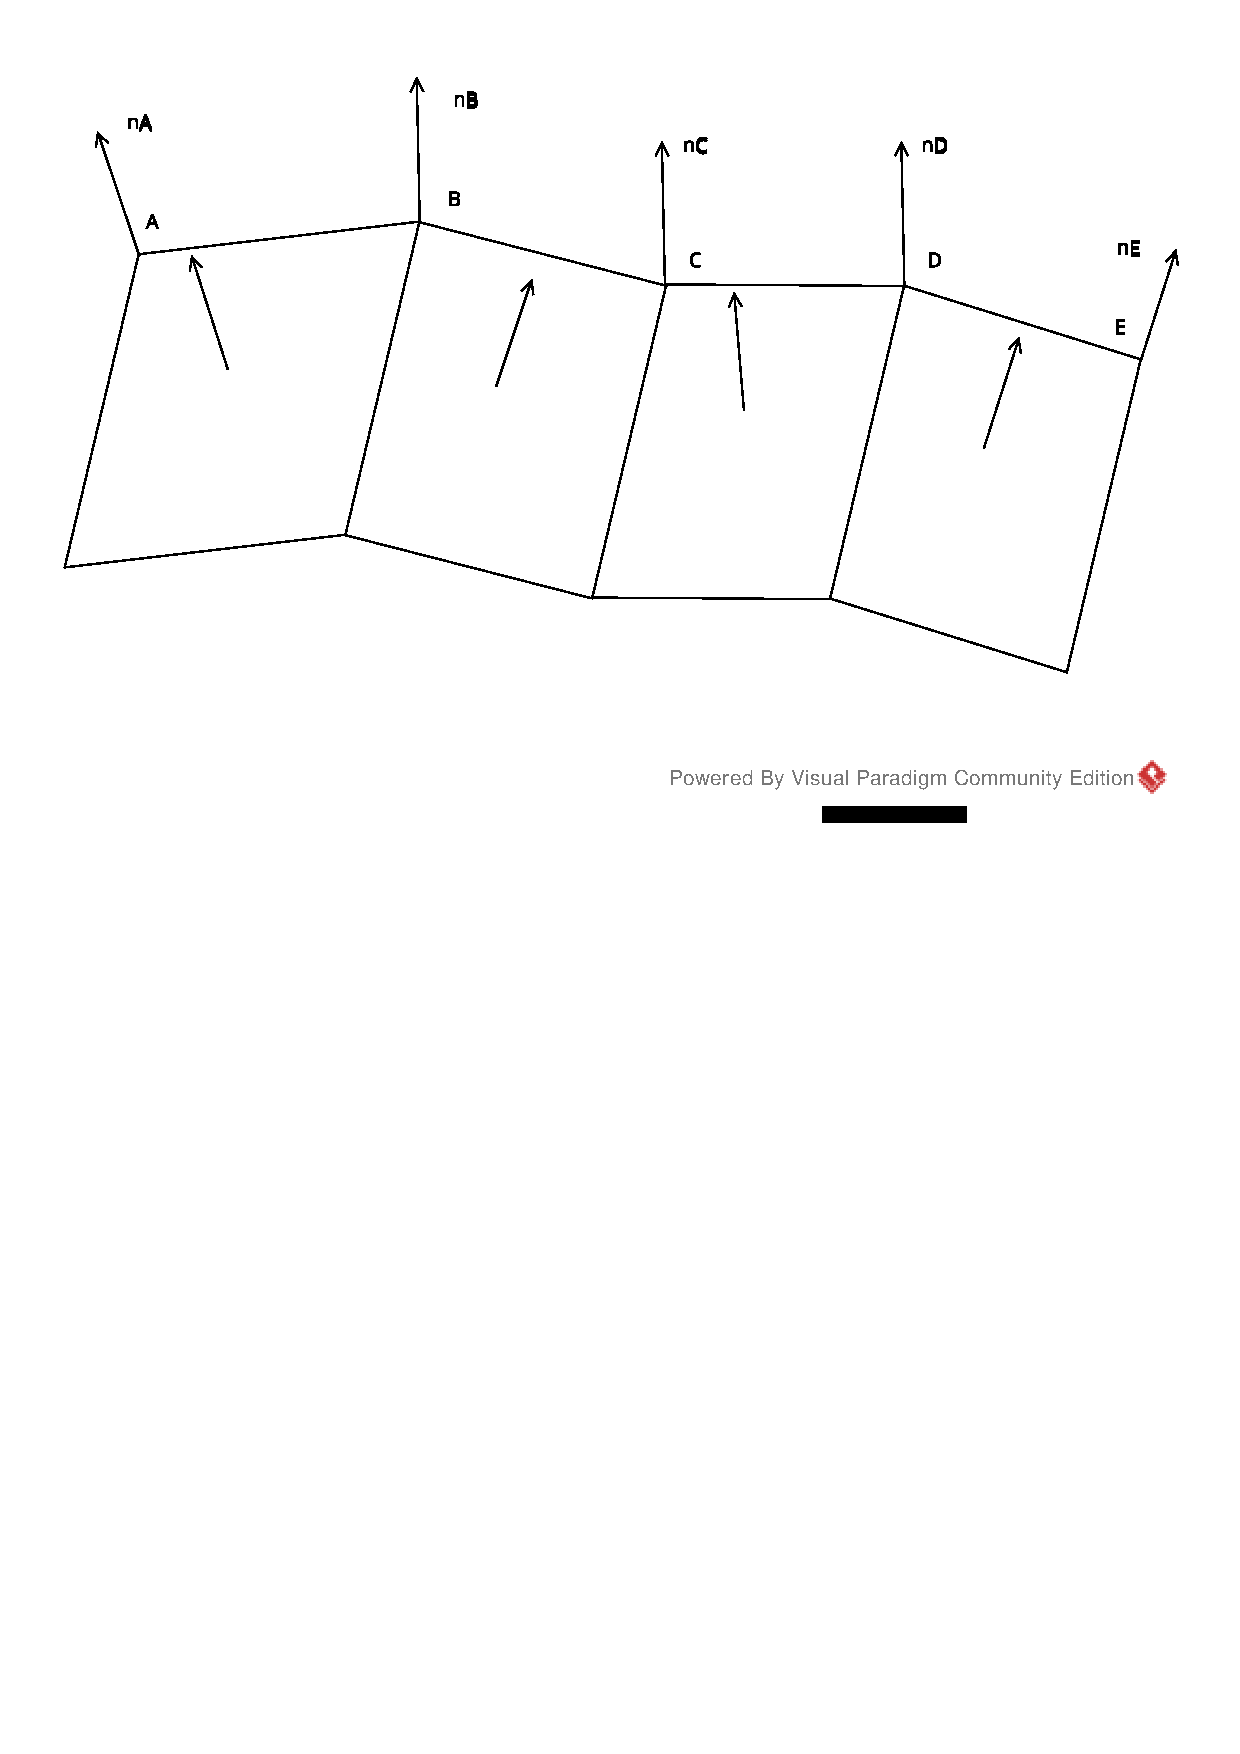
\includegraphics[width=1.0\textwidth]{Knizhka.pdf}
	\caption{Пример некорректной работы закраски Гуро}
	\label{fig:Guro_book}
\end{figure}

\subsection{Закраска методом Фонга}
Фонг предложил вместо интерполяции интенсивностей произвести интерполяцию вектора нормали к поверхности на сканирующей строке. Этот метод требует больших вычислительных затрат, поскольку формулы интерполяции применяются уже к трем компонентам вектора нормали, но зато дает лучшую аппроксимацию кривизны поверхности. Поэтому зеркальные свойства поверхности воспроизводятся гораздо лучше.

Нормали к поверхности в вершинах многогранника вычисляются так же, как и в методе Гуро, после чего выполняется билинейная интерполяция в сочетании с построчным сканированием. После построения вектора нормали в очередной точке вычисляется интенсивность \cite{lit5}.

\section{Построение теней}
Тени делятся на два вида: собственные и проекционные. Определение собственных теней не представляет сложностей: точка наблюдателя совмещается с положением источника света и решается задача определения видимых граней. Видимые грани окажутся освещенными, невидимые -- в тени.

Если источник света находится на бесконечном расстоянии, то при падении света на объект сцены будет образовываться полоса тени, которую можно задать уравнением. Если же источник света находится не на бесконечном расстоянии, возникает потребность нахождения проекции грани в тени на поверхность другого тела \cite{lit6}.

Стоит отметить, что в случае алгоритма обратной трассировки лучей задача построения теней сводится к тому, чтобы при нахождении точки пересечения луча с объектом сцены провести еще один луч от этой точки к источнику света. Если на пути луча встречается преграда в виде поверхности какого-либо объекта сцены, точка находится в тени.


\subsection*{Вывод}

В данном разделе были рассмотрены основные методы построения реалистичных изображений. Для удаления невидимых ребер, учета отражения света и теней в данной работе был выбран алгоритм обратной трассировки лучей в силу своей универсальности и реалистичности результата.

\clearpage
